%
\section{Grouping and labeling}
%
% Remember to mention that video quality isn't used after phase 1 due to the side effects cased by labeling the video (namely that bad quality segments don't receive any labels). in a real world application this quality measure could be used to reduce the amount of data to analyze

%
\subsection{Literature Study}
%
% describe Haar cascade classifiers (performance and an outline of how they work)
Detecting suitable regions in the video-clips is not enough. The content in the regions also has to be interesting. Hanjalic, A. \cite{citeulike:405480} describes a way to identify such regions by measuring the level of excitement in a sports video-clip based on a manually selected set of features. These features can be both visuals (like the movement in an image or the change of camera positions) or audial (namely the energy contained in the audio track).% WHETHER SUCH AN APPROACH IS SUITABLE TO US IS YET TO BE DETERMINED BASED ON THE CONTENT IN OUR FUTURE DATA SET.
%
\subsection{Method}
%
% how we implemented the Haar cascade classifier

%
\subsection{Detecting interesting regions in video-clips}
%

%
\subsection{Metadata}
%

%
\subsubsection{Facial Detection}
%
% using haar cascade classifier
% profile, standard and upper body

%
\subsubsection{Brightness}
%

%
\subsubsection{Optical Flow}
%

%
\subsubsection{Blue channel}\label{sec:blue_channel}
%
Each frame in a video consists of a matrix of pixels in 3 channels, red, green, and blue. For the purpose of police detection, described in detail in section \ref{sec:police_detection}, and day/night detection, described in detail in section \ref{blah}, we extracted the blue channel in each frame and computed the mean pixel intensity. 
%
\subsubsection{Contrast}
%
% from phase1

%
\subsubsection{Shift Vector Magnitude}
%
% from phase1

%
\subsection{Labels}
%

%
\subsubsection{Police Detection}\label{sec:police_detection}
%
% blue channel mean, local minima/maxima. oscillation
By investigating the blue channel mean, see section \ref{sec:blue_channel}, in detail we are able to some degree detect if the police is present in part of a video, under the circumstance that the police blinker lights are active. The theory was simple: we would expect the blue channel mean to oscilate over time. If we plot the mean values as a function of time (frames) we can easily distinguish oscilating areas visually, and then check if this osciallation corresponds to police being present in the video at that point in time. Somewhat to our surprise this was amazingly accurate. We did get a rather large number of false negatives, but almost no false positives.\\
We did not find any ready-at-hand code for detecting oscillations so we rolled something ourselves. What we ended up with was a simple approach based on the realization that the points in an oscillating graph could be connected by triangular shapes (bottom facing up) see Figure \ref{fig:triangles}, and each consequtive triangle is roughly the same shape and size. The problem was boiled down to matching these triangles.\\
We compute the magnitude of the vectors a,b,c,d,e,f and check if the relative standard deviation of $[a,b,c,d]$ and $[e,f]$ is below a certain treshold (meaning that a,b,c,d and e,f are roughly the same length).
%
\begin{figure}
     \centering
     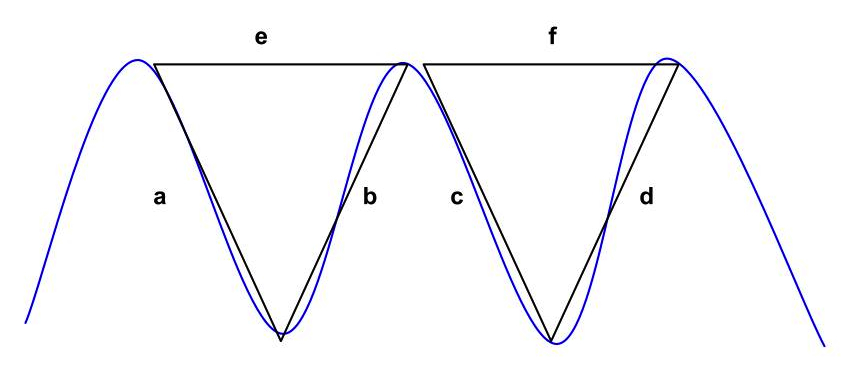
\includegraphics[width=1.05\textwidth]{img/triangles.jpg}
     \caption{}\label{fig:triangles}
\end{figure}
% 
%
\subsubsection{Vertical Oscillation}
%

%
\subsubsection{In crowd}
%
% based on facial detection

%
\subsubsection{Person in Focus}
%
% based on facial detection and object placement in frame (center)

%
\subsubsection{Overview}
%

%
\subsubsection{Day \& Night}
%
% Test/Success-rate